\chapter{Omówienie architektury modułu ESP8266}
\label{omowienie_arch}

\section{Opis modułu}
\label{opis_modulu}

ESP8266 jest tanim modułem umożliwiającym komunikację przez Wi-Fi.
Oferuje on pełną obsługę protokołu TCP/IP a także funkcjonalność prostego
32 bitowego mikrokontrolera. Jest naturalnym następcą modułu ESP32. Niska cena 
i mały rozmiar sprawiły że stał się on bardzo popularny wśród konstruktorów 
urządzeń internetu rzeczy.\\

\begin{figure}[H]
	\centering
    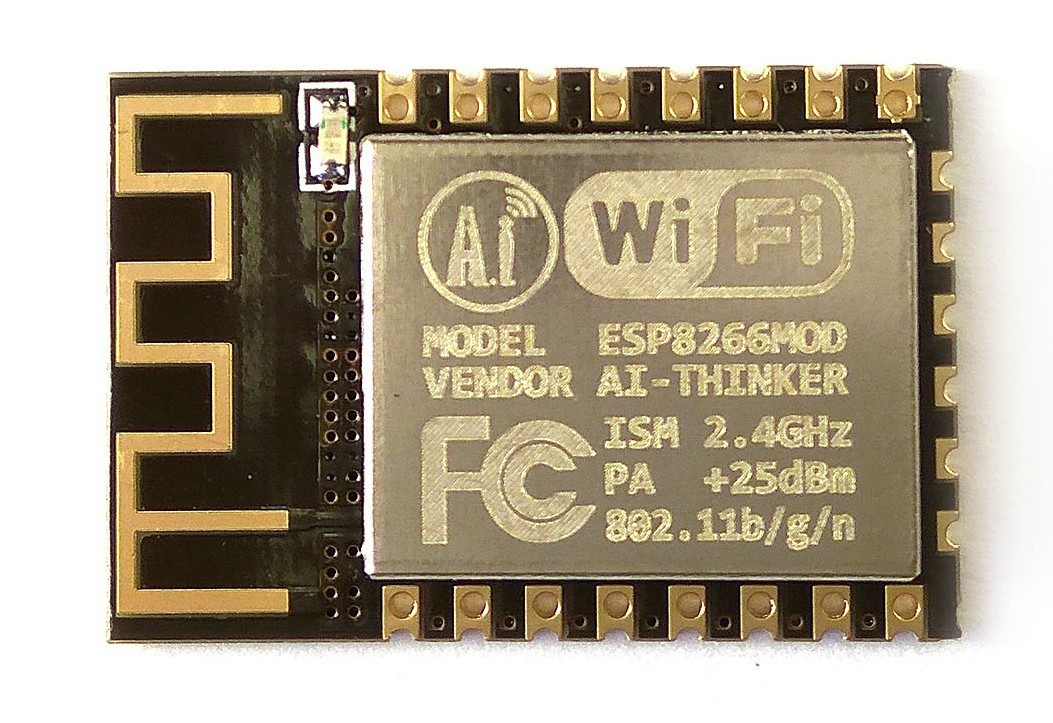
\includegraphics[width=8cm]{./images/esp8266.jpg}
    \caption{Moduł ESP8266 w podstawowej wersji ESP8266-12F firmy AI Thinker}
	\label{esp8266}
\end{figure}

\subsection{Mikroprocesor}
\label{mikroprocesor}

Na pokładzie modułu ESP8266 znajduje się 32 bitowy mikroprocesor z architektury RISC, 
bazowany na standardzie Xtensa Diamond Standard 106Micro firmy Tensilica.
Jest on domyślnie taktowany zegarem $\num{80}$ MHz, którego częstotliwość można 
zwiększyć do $\num{160}$ MHz. Mikroprocesor został tak skonstruowany aby pobierać 
możliwie jak najmniej energii, przez co dostępne są trzy tryby pracy:
\begin{itemize}
    \item \textit{active mode} 
    \item \textit{sleep mode}
    \item \textit{deep sleep mode}
\end{itemize}
W trybie \textit{deep sleep mode} moduł pobiera około $\num{60}$ \si{\micro A}, co pozwala
na bardzo długą pracę urządzenia zasilanego z baterii.


\subsection{Organizacja pamięci}
\label{pamiec}
Moduł ESP8266 został wyposażony w wbudowaną pamięc SRAM oraz ROM. Rozmiar dostępnej
pamięci RAM dla programu użytkownika w przypadku podłączenia do sieci Wi-Fi w trybie
\textit{station mode} wynosi około $\num{80}$ KiB. Docelowo 
pamięc RAM dostępna dla użytkownika rozpoczyna się od adresu \texttt{3FFE8000h}.
Ten obszar pamięci służy do przechowywania aktualnie obrabianych danych, jest to typowa 
pamięć operacyjna modułu.
Wewnętrzna pamięć ROM nie jest programowalna a jej rozmiar wynosi $\num{64}$ KiB.
Pamięć ROM mapowana jest w taki sposób że rozpoczyna się od adresu \texttt{40000000h}.
W pamięci ROM znajduje się bootloader, który obsługuje pobieranie nowego programu poprzez
UART oraz jego wykonywaniem z pamięci Flash, a także implementacja podstawowych funkcji typu
\texttt{alloc} czy \texttt{memcpy}.

\begin{figure}[H]
	\leftskip3cm
    \includegraphics[width=8cm]{./images/memorymap.pdf}
    \caption{Uproszczona mapa pamięci modułu ESP8266}
	\label{memmap}
\end{figure}

Oprócz wbudowanej pamięci, na pokładzie modułu znajduje się również zewnętrzna programowalna
pamięć Flash do przechowywania programów użytkownika. Według dokumentacji, istnieje
możliwość podłączenia pamięci o maksymalnym rozmiarze $\num{16}$ MiB. Zakłada się 
że minimalny rozmiar pamięci Flash powinien wynosić $\num{512}$ KiB w przypadku wyłaczonej
funkcjonalności OTA (Over The Air Update) i $\num{1}$ MiB przy włączonym OTA. Komunikacja
z pamięcią Flash zachodzi przy pomocy interfejsu SPI.

\subsection{Wi-Fi}
\label{wifi}
Głównym zastosowaniem modułu ESP8266 jest możliwość komunikowania się urządzenia wbudowanego
z siecią Wi-Fi. Urządzenie oparte na ESP8266 może pełnić trzy role w sieci:\\
\begin{itemize}
    \item \textit{Wireless Access Point (AP)}
    \item \textit{Station}
    \item \textit{AP + Station}\\
\end{itemize}

\textit{Wireless Access Point}, w skrócie AP, to urządzenie które pełni rolę 
hubu komunikacyjnego.  To z AP łączą się urządzenia nazywane stacjami (z ang. \textit{Station}).
AP są najczęściej połączone z internetem, co umożliwia stacjom
bezprzewodowe połaczenie z siecią. ESP8266 może pełnić obie role, wymiennie oraz równocześnie.\\

\begin{figure}[H]
	\centering
    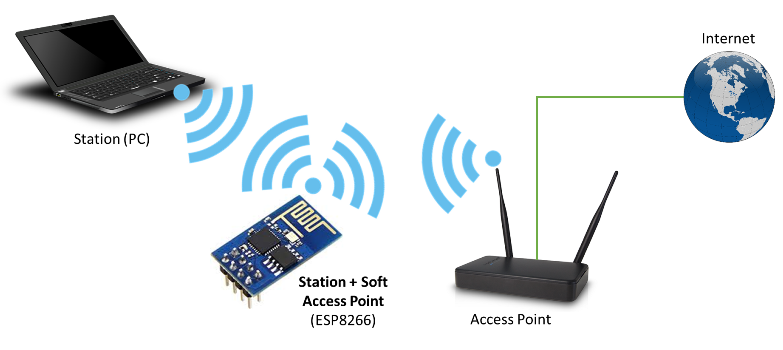
\includegraphics[width=12cm]{./images/WiFi-stationap-mode.png}
    \caption{Praca modułu ESP8266 jako \textit{Access Point} oraz jako \textit{Station}}
    \label{ap+station}
\end{figure}


Komunikacja sieciowa jest obsługiwana przez wewnętrzny kod. Stawia to pewne ograniczenia 
na program użytkownika, wynikające z faktu że w trakcie wykonywania kodu aplikacji 
użytkownika, nie jest wykonywany kod obsługujący komunikację. Brak wątków powoduje że 
kod użytkownika zawsze przerywa obsługę zdarzeń sieciowych. Aby umożliwić poprawne działanie
modułu, należy tak zaprojektować kod użytkownika aby pojedyncze wejście do kodu użytkownika
trwało krócej niż $\num{10}$ ms.\\


Moduł ESP8266 docelowo przechowuje informację o sieci z którą ma się połączyć w pamięci Flash.
Umożliwia to połączenie się z siecią po restarcie urządzenia bez żadnych dodatkowych informacji 
z zewnątrz. Znacznie upraszcza to uruchamianie urządzenia, jednak powoduje że zmiana sieci 
lub tylko hasła do niej wymaga przeprogramowania pamięci. Istnieje jednak możliwość 
nadpisania funkcji automatycznie łączących się z AP \verb+wifi_station_set_auto_connect()+ oraz 
\verb+wifi_station_get_auto_connect()+, tak aby po restarcie pobierały one dane z interfejsu szeregowego.\\

W przypadku pracy w trybie \textit{Station}, urządzenie skanuje dostępne sieci
bezprzewodowe z którymi może się połączyć. Do skanowania została przygotowana 
funkcja \verb+wifi_station_scan()+, która jako argument przyjmuję \textit{callback}
do której jako argument zostanie przekazana lista struktur BSS. Struktura BSS
przechowuje informację o SSID sieci, BSSID powiązanego z danym AP, kanale, mocy
sygnału i wielu innych. Na samym końcu struktury znajduje się wskaźnik na następny 
element listy.\\

Obsługa zdarzeń sieciowych również opiera się na \textit{callback'ach}. Za pomocą 
funkcji \verb+wifi_set_event_handler_cb()+, możemy ustawić która funkcja ma 
obsługiwać zdarzenia sieciowe. Poniżej przedstawiono postać przykładowej funkcji.\\

\begin{lstlisting}[style=customc,
    frame=single,
    caption={Przykładowa postać funkcji obsługującej zdarzenia sieciowe},
    captionpos=b,
    label={event_handler_cb}]
void eventHandler(System_Event_t *event) {
    switch(event->event) {
      case EVENT_STAMODE_CONNECTED:
        os_printf("Event: EVENT_STAMODE_CONNECTED\n");
        break;
      case EVENT_STAMODE_DISCONNECTED:
        os_printf("Event: EVENT_STAMODE_DISCONNECTED\n");
        break;
      default:
        os_printf("Unexpected event: %d\n", event->event);
        break;
    }
}
\end{lstlisting}

\subsection{Interfejsy zewnętrzne}
\label{interfejsy}

\subsubsection{GPIO}
\label{gpio}
Moduł ESP8266 oferuje do 17 typowych pinów wejścia-wyjścia ogólnego przeznaczenia. Piny
te są multipleksowane z innymi funkcjami takimi jak I2C czy PWM, opisanymi w dalszej 
części tego dokumentu. Wszystkie piny mogą zostać skonfigurowane z wewnętrznym 
podciągnięciem do zasilania (\textit{pull-up}), w konfiguracji \textit{push-pull} lub 
\textit{open-drain}. Można skonfigurować piny w taki sposób aby zmiana zbocza zgłaszała
przerwanie do procesora.


\subsubsection{SDIO}
\label{sdio}
Moduł oferuje jeden interfejs \textit{Secure Digital Input Output}, który wykorzystywany
jest do komunikacji z kartami SD a także z innymi urządzeniami obsługującymi ten standard.


\subsubsection{SPI}
\label{spi}
W ESP8266 znalazło się miejsce na sprzętowy interfejs SPI. Możliwe jest połączenie się z jednym
urządzeniem jako master lub jako slave.


\section{Organizacja oprogramowania}
\label{organizacja_opr}